%me=0 student solutions (ps file), me=1 - my solutions (sol file), me=2 - assignment (hw file)
\def\me{0}
\def\num{2}  %homework number
\def\due{Tuesday, September 22}  %due date
\def\course{CSCI-GA.1170-001/002 Fundamental Algorithms} %course name, changed only once
\def\name{GOWTHAM GOLI (N17656180)}   %student changes (instructor keeps!)
%
\iffalse
INSTRUCTIONS: replace # by the homework number.
(if this is not ps#.tex, use the right file name)

  Clip out the ********* INSERT HERE ********* bits below and insert
appropriate TeX code.  Once you are done with your file, run

  ``latex ps#.tex''

from a UNIX prompt.  If your LaTeX code is clean, the latex will exit
back to a prompt.  To see intermediate results, type

  ``xdvi ps#.dvi'' (from UNIX prompt)
  ``yap ps#.dvi'' (if using MikTex in Windows)

after compilation. Once you are done, run

  ``dvips ps#.dvi''

which should print your file to the nearest printer.  There will be
residual files called ps#.log, ps#.aux, and ps#.dvi.  All these can be
deleted, but do not delete ps1.tex. To generate postscript file ps#.ps,
run

  ``dvips -o ps#.ps ps#.dvi''

I assume you know how to print .ps files (``lpr -Pprinter ps#.ps'')
\fi
%
\documentclass[11pt]{article}
\usepackage{amsfonts}
\usepackage{latexsym}
\usepackage[lined,boxed,linesnumbered]{algorithm2e}
\usepackage{amsmath}
\usepackage{amssymb}
\usepackage{amsthm}
\usepackage{epsfig}
\usepackage{psfrag}
\usepackage{color}
\usepackage{tikz}
\usetikzlibrary{trees}
\usepackage{mathtools}
\usepackage{float}
\setlength{\oddsidemargin}{.0in}
\setlength{\evensidemargin}{.0in}
\setlength{\textwidth}{6.5in}
\setlength{\topmargin}{-0.4in}
\setlength{\textheight}{8.5in}

\newcommand{\handout}[5]{
   \renewcommand{\thepage}{#1, Page \arabic{page}}
   \noindent
   \begin{center}
   \framebox{
      \vbox{
    \hbox to 5.78in { {\bf \course} \hfill #2 }
       \vspace{4mm}
       \hbox to 5.78in { {\Large \hfill #5  \hfill} }
       \vspace{2mm}
       \hbox to 5.78in { {\it #3 \hfill #4} }
      }
   }
   \end{center}
   \vspace*{4mm}
}

\newcounter{pppp}
\newcommand{\prob}{\arabic{pppp}}  %problem number
\newcommand{\increase}{\addtocounter{pppp}{1}}  %problem number

%first argument desription, second number of points
\newcommand{\newproblem}[2]{
\ifnum\me=0
\ifnum\prob>0 \newpage \fi
\increase
\setcounter{page}{1}
\handout{\name, Homework \num, Problem \arabic{pppp}}{\today}{Name: \name}{Due:
\due}{Solutions to Problem \prob\ of Homework \num\ (#2)}
\else
\increase
\section*{Problem \num-\prob~(#1) \hfill {#2}}
\fi
}

%\newcommand{\newproblem}[2]{\increase
%\section*{Problem \num-\prob~(#1) \hfill {#2}}
%}

\def\squarebox#1{\hbox to #1{\hfill\vbox to #1{\vfill}}}
\def\qed{\hspace*{\fill}
        \vbox{\hrule\hbox{\vrule\squarebox{.667em}\vrule}\hrule}}
\newenvironment{solution}{\begin{trivlist}\item[]{\bf Solution:}}
                      {\qed \end{trivlist}}
\newenvironment{solsketch}{\begin{trivlist}\item[]{\bf Solution Sketch:}}
                      {\qed \end{trivlist}}
\newenvironment{code}{\begin{tabbing}
12345\=12345\=12345\=12345\=12345\=12345\=12345\=12345\= \kill }
{\end{tabbing}}

%\newcommand{\eqref}[1]{Equation~(\ref{eq:#1})}
\newcommand\quest{\mathrel{\overset{\makebox[0pt]{\mbox{\normalfont\tiny\sffamily ?}}}{\leq}}}
\newcommand\ind{\mathrel{\overset{\makebox[0pt]{\mbox{\normalfont\tiny\sffamily ind}}}{\leq}}}


\newcommand{\hint}[1]{({\bf Hint}: {#1})}
%Put more macros here, as needed.
\newcommand{\room}{\medskip\ni}
\newcommand{\brak}[1]{\langle #1 \rangle}
\newcommand{\bit}[1]{\{0,1\}^{#1}}
\newcommand{\zo}{\{0,1\}}
\newcommand{\C}{{\cal C}}

\newcommand{\nin}{\not\in}
\newcommand{\set}[1]{\{#1\}}
\renewcommand{\ni}{\noindent}
\renewcommand{\gets}{\leftarrow}
\renewcommand{\to}{\rightarrow}
\newcommand{\assign}{:=}

\newcommand{\AND}{\wedge}
\newcommand{\OR}{\vee}

\newcommand{\Forr}{\mbox{\bf For }}
\newcommand{\To}{\mbox{\bf to }}
\newcommand{\Do}{\mbox{\bf Do }}
\newcommand{\Ifi}{\mbox{\bf If }}
\newcommand{\Thenn}{\mbox{\bf Then }}
\newcommand{\Elsee}{\mbox{\bf Else }}
\newcommand{\Whilee}{\mbox{\bf While }}
\newcommand{\Repeatt}{\mbox{\bf Repeat }}
\newcommand{\Until}{\mbox{\bf Until }}
\newcommand{\Returnn}{\mbox{\bf Return }}
\newcommand{\Swap}{\mbox{\bf Swap }}



\begin{document}

\ifnum\me=0
%\handout{PS\num}{\today}{Name: **** INSERT YOU NAME HERE ****}{Due:
%\due}{Solutions to Problem Set \num}
%
%I collaborated with *********** INSERT COLLABORATORS HERE (INDICATING
%SPECIFIC PROBLEMS) *************.
\fi
\ifnum\me=1
\handout{PS\num}{\today}{Name: Yevgeniy Dodis}{Due: \due}{Solution
{\em Sketches} to Problem Set \num}
\fi
\ifnum\me=2
\handout{PS\num}{\today}{Lecturer: Yevgeniy Dodis}{Due: \due}{Problem
Set \num}
\fi




\newproblem{Different Methods for Recurrences}{14 points}



Consider the recurrence $T(n) = 8T(n/4) + n$ with initial condition
$T(1)=1$.

\begin{itemize}

\item[(a)] (2 points) Solve it asymptotically using the ``master theorem''.

\ifnum\me<2
\begin{solution}

From Master Theorem, $a = 8, b = 4$ and $f(n) = n$\\
\begin{align*}
f(n) &= n\\
\implies f(n) &= O(n^{\log_4 (8-4)})\\
\implies f(n) &= O(n^{\log_b (a-\epsilon)})\,\,\,\, with \,\,\,\, \epsilon > 0\\
\implies T(n) &= \Theta(n^{\log_b a})\\
\therefore T(n) &= \Theta(n^{\log_4 8})\\
&= \Theta(n^{3/2})
\end{align*}
\end{solution}
\fi

\item[(b)] (4 points) Solve it by the ``guess-then-verify method''. Namely, guess a
function $g(n)$ --- presumably solving part (a) will give you a good
guess --- and argue by induction that for all values of $n$ we have
$T(n) \le g(n)$. What is the ``smallest'' $g(n)$ for which your
inductive proof works?

\ifnum\me<2
\begin{solution}

\textbf{Guess} -  $T(n) \leq cn^{3/2}$\\
\textbf{Base Case} - $1= T(1) \quest c(1)^{3/2} = c \implies c \geq 1$\\
\textbf{Induction} -  $T(n) = 8T(n/4) + n \ind 8(c(n/4)^{3/2}) + n = cn^{3/2} + n \quest cn^{3/2} \implies$ not valid

$\therefore$ Our guess must be wrong. Hence we need to make another guess

\textbf{Next Guess} - $T(n)  \leq cn^{3/2} - dn$\\
\textbf{Base Case} - $1 = T(1) \quest c(1)^{3/2}- d(1)  = c-d \implies  c \geq d+1$\\
\textbf{Induction} - $T(n) = 8T(n/4) + n \leq 8(c(n/4)^{3/2} - d(n/4)) = cn^{3/2} - 2dn + n \quest cn^{3/2}-dn \\ \implies d \geq 1$ and $ c \geq 2, \,\, \forall n \geq 2 $

In the ideal case, $cn^{3/2} - dn$ has to be smallest $\implies c$ has to be smallest and $d$ has to be greatest. But we give more importance to $c$ being smaller as $c$ is attached to $n^{3/2}$.\\
$\therefore$  $\,\,\,$   for $d = 1,\,\,\, c \geq 1+1 = 2$ 

Hence the smallest $g(n)$ for which the inductive proofs works is $2n^{3/2}-n$

\end{solution}
\fi

\item[(c)] (4 points) Solve it by the ``recursive tree method''. Namely, draw the
full recursive tree for this recurrence, and sum up all the value to
get the final time estimate. Again, try to be as precise as you can
(i.e., asymptotic answer is OK, but would be nice if you preserve a
``leading constant'' as well).

\ifnum\me<2
\begin{solution}
\begin{figure}[H]
	\centering
	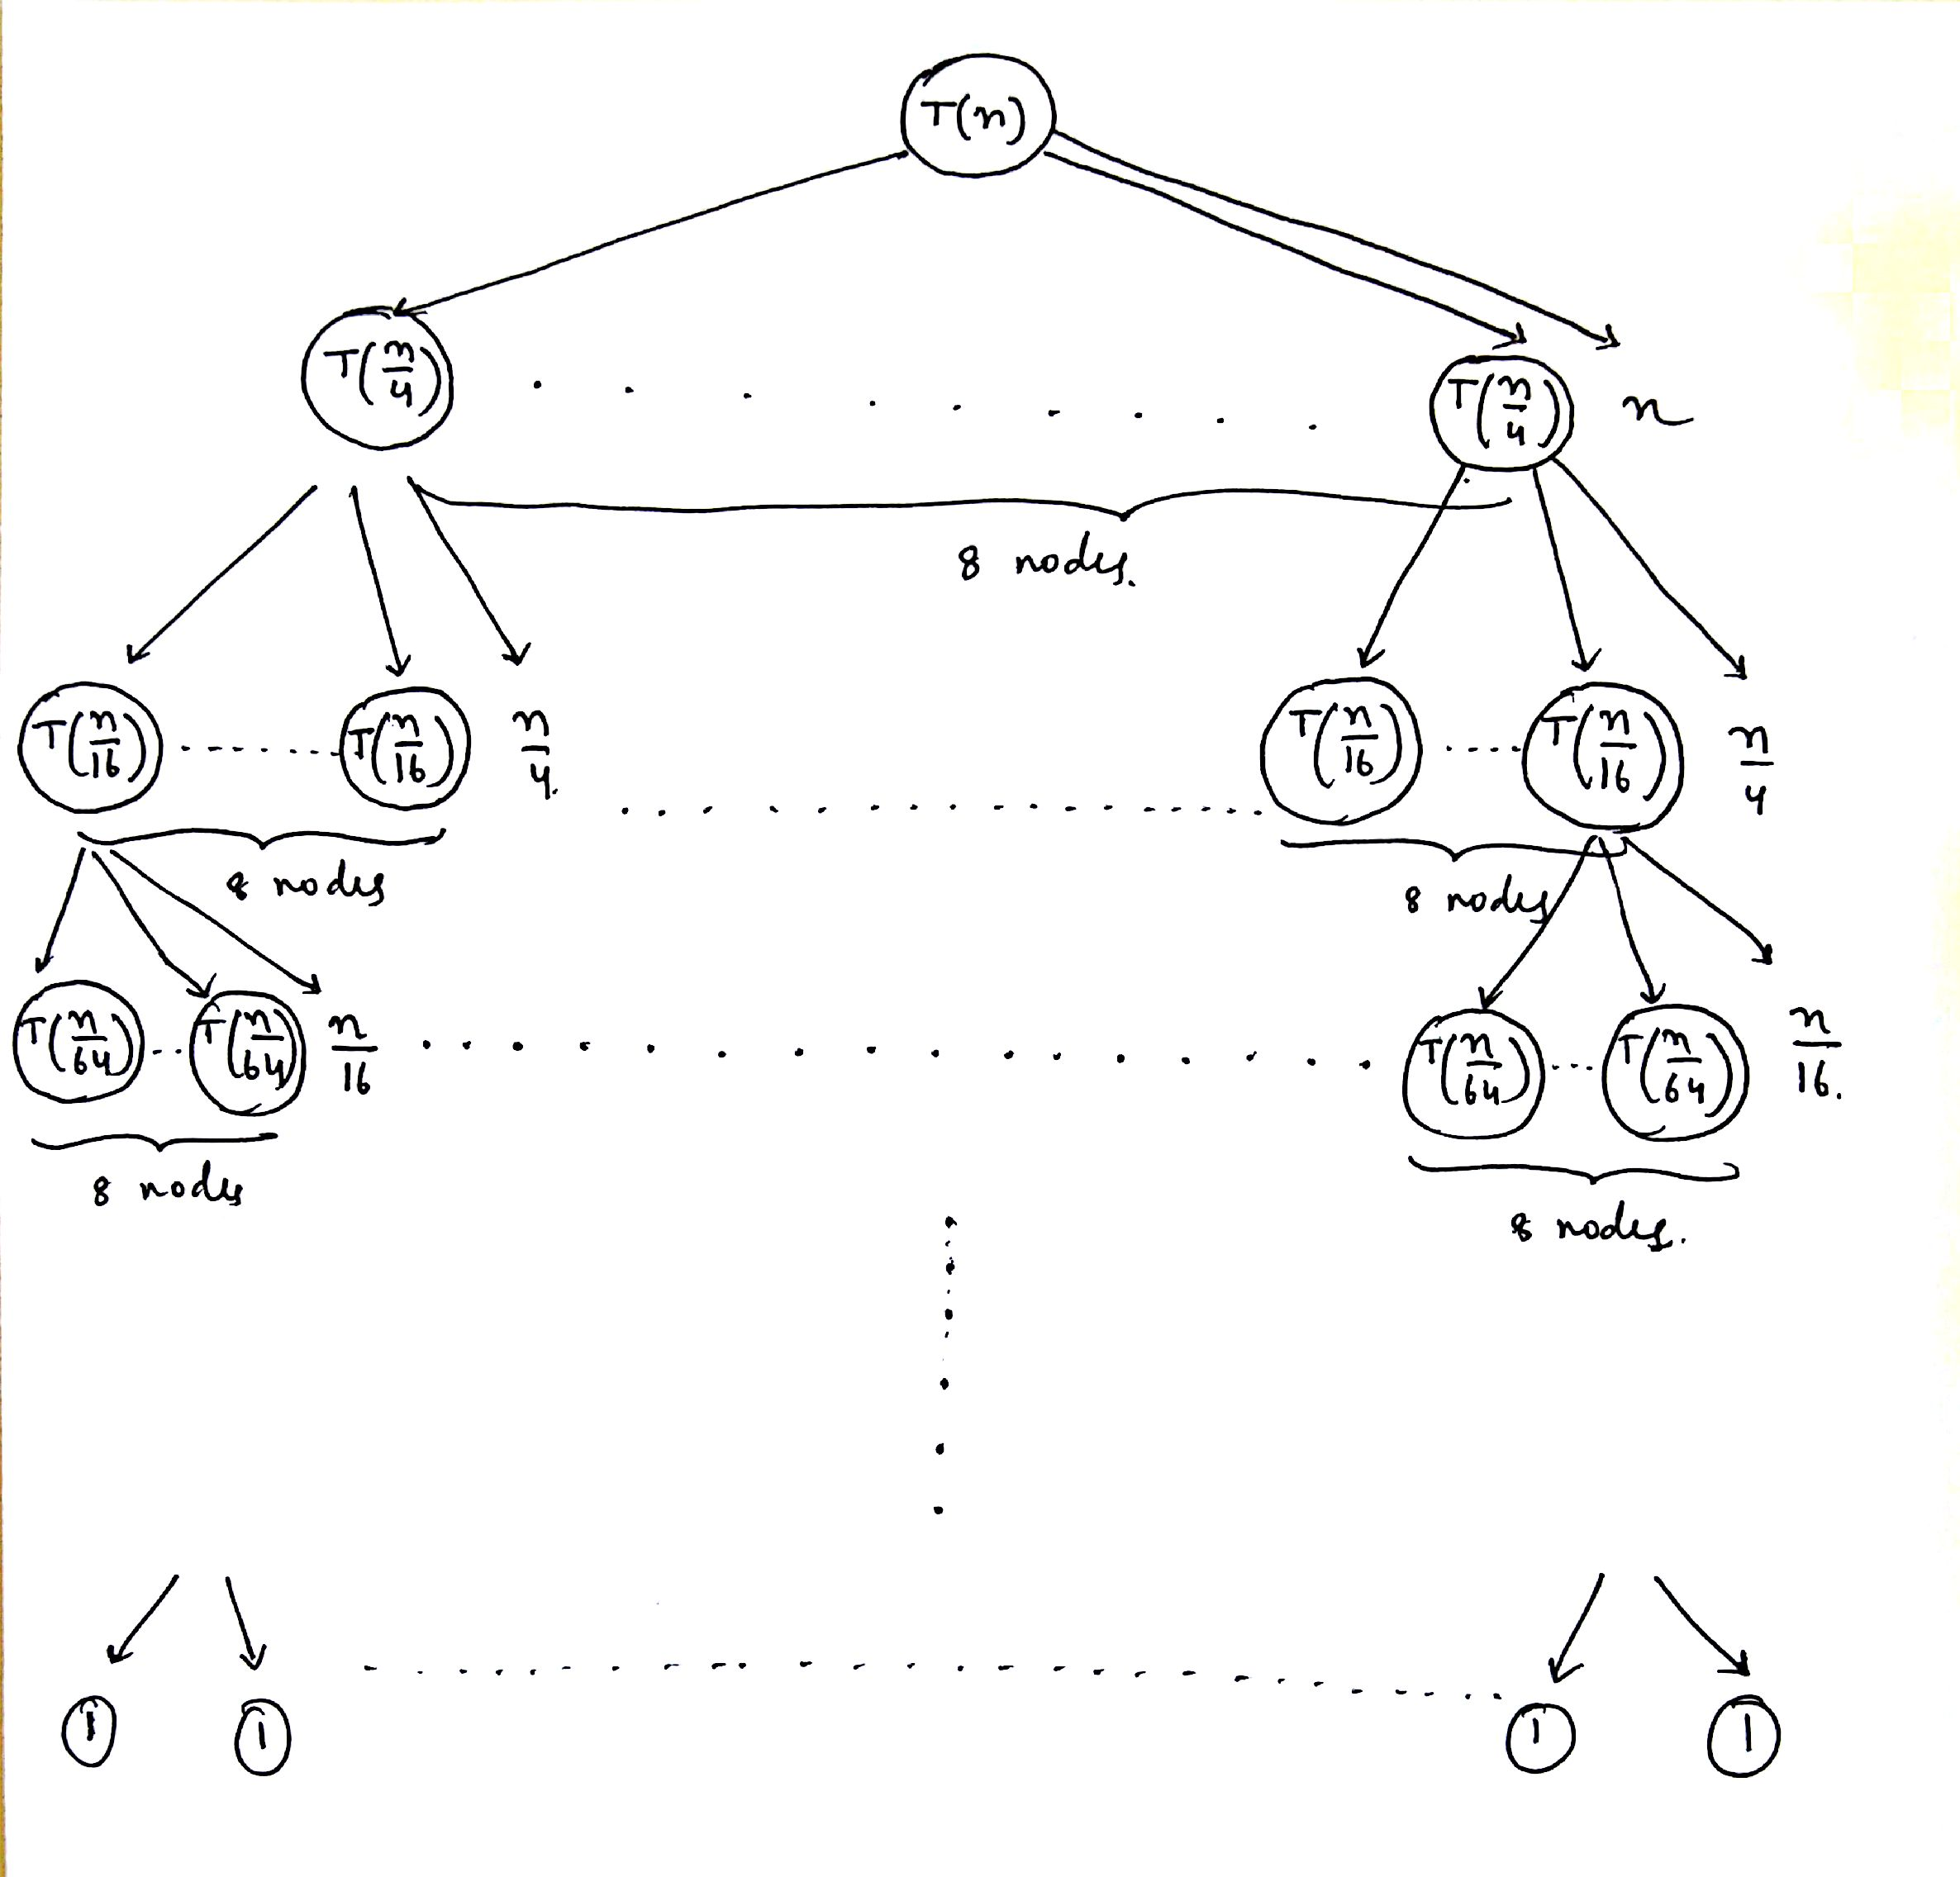
\includegraphics[width=0.95\columnwidth]{recursive.jpg}
	\caption{Recursive Tree of $T(n)$}
	\label{1}
\end{figure}
\clearpage
Work done in first level is $n$\\
Work done in second level is $8(n/4) = 2n$ \\
Work done in third level is $64(n/16) = 4n$\\
$\vdots$\\
Work done in $k^{th}$ level is $2^{k-1}n$

Height of tree = $\log_4 n = \log_2 \sqrt{n}$

$\therefore$ Total number of computations is\\
\begin{align*}
\Sigma_k &= n + 2n + 4n + \ldots + 2^{k-1}n\\
&= n(1+2+4+ \ldots+ 2^{k-1})\\
&= n(\frac{2^k-1}{2-1})\\
&= n(2^k-1)\\
\implies \Sigma_{\log \sqrt{n}} &= n(2^{\log n^{\frac{1}{2}}} - 1)\\
&= n(n^{1/2}-1)\\
\therefore T(n) &= n^{3/2} -n\\
&= \Theta(n^{3/2} -n)
\end{align*}

\end{solution}
\fi

\item[(d)] (4 points) Solve it {\em precisely} using the ``domain-range
substitution'' technique. Namely, make several changes of variables
until you get a basic recurrence of the form $S(k) = S(k-1) + f(k)$
for some $f$, and then compute the answer from there. Make sure you
carefully maintain the correct initial condition.

\ifnum\me<2
\begin{solution}
Let $n = 4^k$
\begin{align*}
T(4^k) &= 8T(4^k/4) + 4^k\\
T(4^k) &= 8T(4^{k-1})+ 4^k\\
Let\,\,\,\, S(k) &= T(4^k) \implies S(0) = 1\\
\implies S(k) &= 8S(k-1) + 4^k\\
\frac{S(k)}{8^k} &= \frac{S(k-1)}{8^{k-1}} + (1/2)^k\\
Let\,\,\,\, P(k) &= \frac{S(k)}{8^k} \implies P(0) = 1\\
P(k) &= P(k-1) + (1/2)^k\\
\implies P(k) &= 2-(\frac{1}{2})^k\\
\implies S(k) &= 2.8^k - 4^k\\
\end{align*}
\begin{align*}
\implies T(4^k) &= 2.(4^k)^{3/2} - 4^k\\
\implies T(n) &= 2n^{3/2} - n
\end{align*}
\end{solution}
\fi

\item[(e)] This part will not be graded. However, briefly describe
your personal comparison of the above 4 methods. Which one was the
fastest? The easiest? The most precise?

\ifnum\me<2
\begin{solution}

The fastest and the easiest technique was to use Master Theorem. The most precise technique was to use Domain-Range substitution
\end{solution}
\fi

\end{itemize}



\newproblem{Functionality vs. running time}{10  points}

Consider the following recursive procedure.

\medskip

\begin{code}
\>{\sc Bla}$(n)$:\\
\> \> \Ifi $n=1$ \Thenn \Returnn $1$\\
\> \> \Elsee \Returnn $\mbox{\sc Bla}(n/3) + \mbox{\sc Bla}(n/3)$
\end{code}

\begin{itemize}

\item[(a)] (3 points)
What function of $n$ does {\sc Bla} compute (assume it is
always called on $n$ which is a power of $3$)?

\ifnum\me<2
\begin{solution}
\begin{figure}[H]
	\centering
	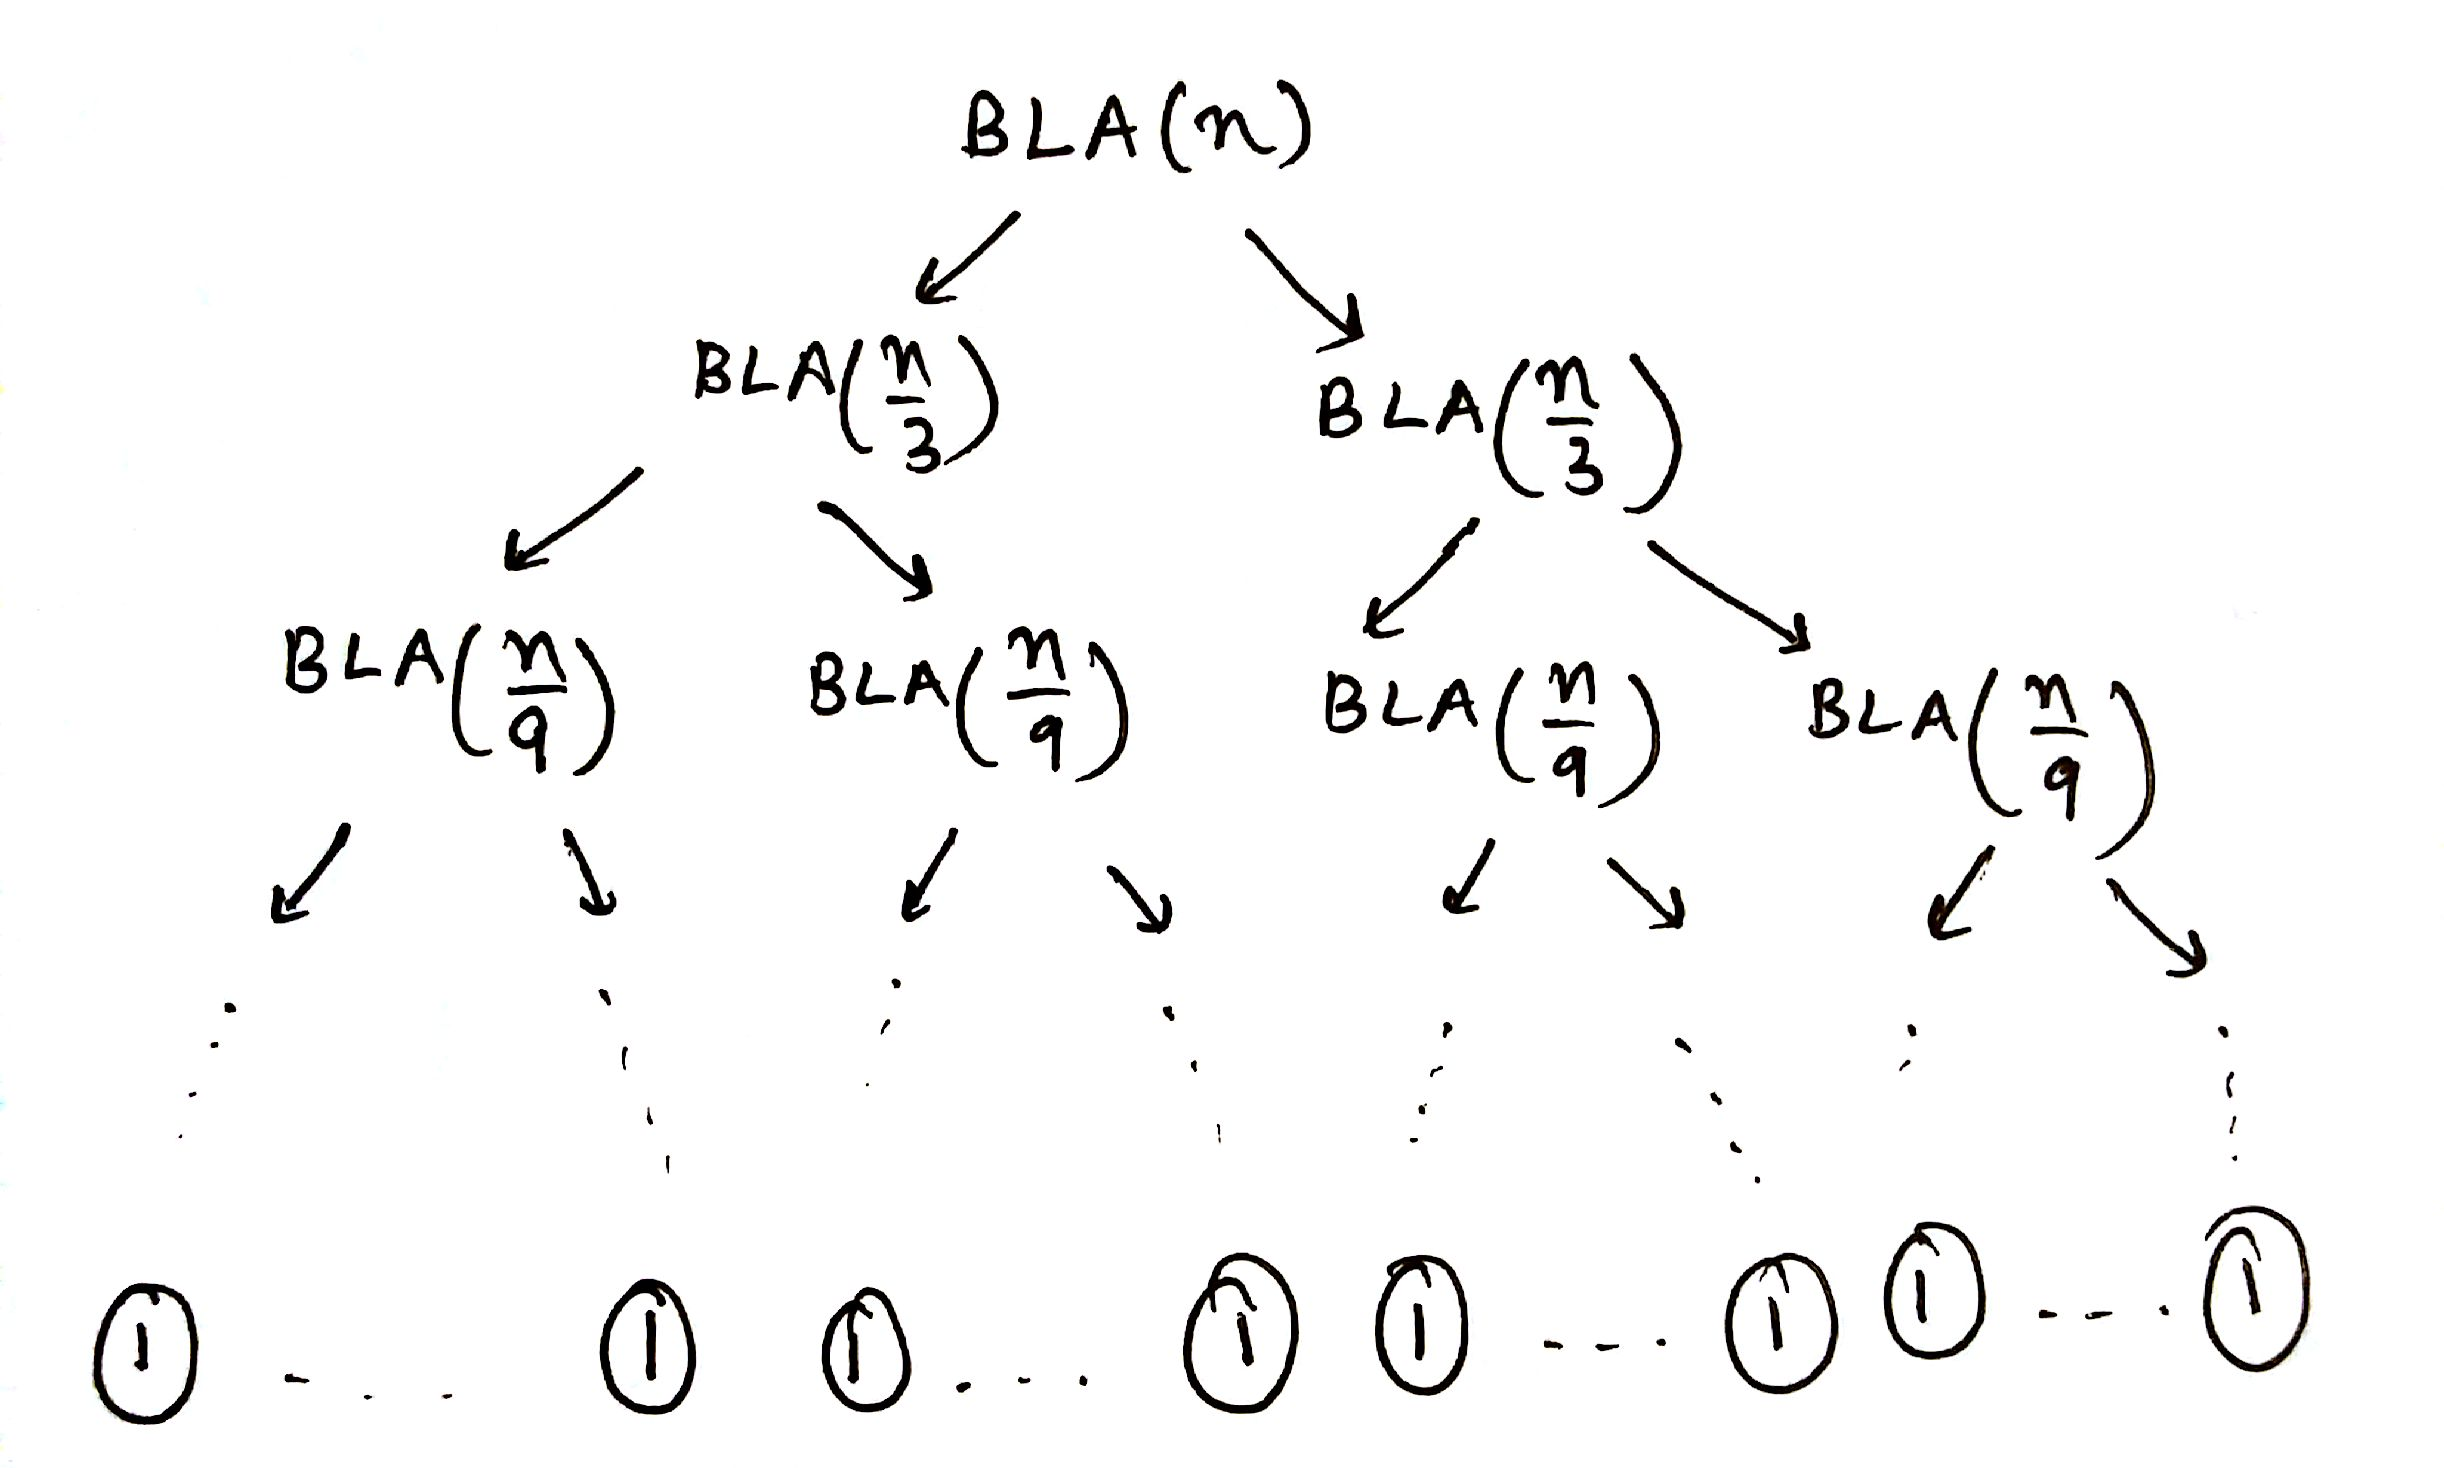
\includegraphics[width=0.95\columnwidth]{bla.jpg}
	\caption{Recursive Tree of $BLA(n)$}
	\label{1}
\end{figure}

In the above tree, at any $k^{th}$ level, number of nodes are $2^k$. The height of the tree is $\log_3 n$. Therefore at the last level, total number of $1's$ returned will be $2^{\log_3 n}$.\\
$\therefore BLA(n) = 2^{\log_3 n}$
\end{solution}
\fi
\pagebreak
\item[(b)] (3 points) What is the running time $T(n)$ of {\sc Bla}?

\ifnum\me<2
\begin{solution}
From the tree, we can see that the recurrence equation will be,
\begin{align*}
T(n) &= 2T(n/3)+1\\
\end{align*}
Using Master Theorem, $a = 2, b = 3$ and $d = 0 \implies d < \log_b a$
\begin{align*}
\therefore T(n) &= O(n^{\log_a b})\\
\implies T(n) &= O(n^{\log_3 2})
\end{align*}
\end{solution}
\fi

\item[(c)] (4 points) How do the answers to (a) and (b) change if we replace the
last line by\\ ``\Elsee \Returnn $2\cdot \mbox{\sc Bla}(n/3)$''?

\ifnum\me<2
\begin{solution}
Answer to part(a) remains the same as computationally $BLA(n/3) + BLA(n/3) = 2BLA(n/3)$\\
However, the answer to part(b) changes as we are reducing the total number of executions by not making a call to $BLA(n/3)$ again and instead, multiplying $BLA(n/3)$ by 2. Therefore, the new recurrence equation will now be\\
\begin{align*}
T(n) &= T(n/3)+1\\
&= T(n/9) + 1 + 1\\
&= \underbrace{1+ 1+ \ldots+1 +1}_{log_3 n \,\,\,\, terms} \\
\implies T(n)&= \log_3 n\\
&= \Theta(\log_3 n)
\end{align*}
\end{solution}
\fi

\end{itemize}


\newproblem{Counting Inversions}{16 points}

Let $A[1 \ldots n]$ be an array of pairwise different numbers. We call
pair of indices $1 \leq i < j \leq n$ an
\emph{inversion} of $A$ if $A[i] > A[j]$. The goal of this problem is
to develop a divide-and-conquer based algorithm running in time
$\Theta(n \log n)$ for computing the number of inversions in $A$.
\begin{itemize}
 \item[(a)] (8 points) Suppose you are given a pair of {\em sorted} integer
 arrays $A$ and $B$ of length $n/2$ each. Let $C$ an $n$-element array
 consisting of the concatenation of $A$ followed by $B$. Give an
 algorithm (in pseudocode) for counting the number of inversions in
 $C$ and analyze its runtime. Make sure you also argue (in English)
 why your algorithm is correct.

\ifnum\me<2
\begin{solution}

Given, $C$ is concatenation of two sorted arrays $A$ and $B$. Therefore, the first half and remaining half of $C$ is sorted (similar to the \textit{Merge} step in \textit{Merge Sort}).

We know that the \textit{Merge} step can be accomplished in $O(n)$ time. Hence by adding some $O(1)$ executions to the \textit{Merge} step, it could be possible to count number of inversions in $O(n)$ time.\\

{\bf Approach}

Let $mid$ be the middle element of $C \implies C[0 \ldots mid]$ and $C[mid+1 \ldots n]$ are sorted.

Therefore, there cannot be any inversions in $C[0 \ldots mid]$ and $C[mid+1 \ldots n]$. The only inversions that can exist in $C$ are the inversions that exist in between the two arrays \\$C[0 \ldots mid]$ and $C[mid+1 \ldots n]$

Let $0 \leq i \leq mid$ and $(mid+1) \leq  j \leq n$. For an inversion to occur,\\ $C[i] > C[j] \implies C[i+1 \ldots mid] > C[j] \,\,\,\,  (\because C[i+1 \ldots mid] > C[i])$

Therefore, the number of inversions will be $mid-i+1$. Then we keep increasing $j$ to find next inversions until it reaches $n$

If $C[i] < C[j] \implies$ this is not an inversion. So we keep increasing $i$ to find an inversion until it reaches $mid$

Hence we can see that the above explained algorithm can be easily included in the \textit{Merge} step just adding a few lines of code.\\

In the following Psuedocode, \textit{Merge\&CountInversions(C, p , mid, k, D)}
\begin{itemize}
\item $p$ is the starting index of $C$ (in this case $p = 0$)

\item $mid$ is the mid-point of $C$

\item $k$ is the length of array $C$ (in this case $c = n$)

\item $D$ is the final sorted array obtained by merging the two halves of $C$
\end{itemize}
$\therefore$ In the main function, \textit{Merge\&CountInversions(C, 0 , mid, k, D)} will be called

\pagebreak
{\bf Pseudo Code}

\IncMargin{1em}
\begin{algorithm}[H]
\TitleOfAlgo{Merge\&CountInversions(C, p , mid, k, D)}
i $\leftarrow$ p ; j $\leftarrow$ mid+1\\
r $\leftarrow$ 0\\
numInversions $\leftarrow$ 0\\

\While{i $\leq$ mid and j $\leq$ n}
{
	\If{C[i] $<$ C[j]}{
		D[r] $\leftarrow$ C[i]\\
		$i$++ ; 
		$r$++
	}
	\Else{
		D[r] $\leftarrow$ C[j] \\
		numInversions = numInversions + $(mid-i+1)$\\
		$j$++ ; 
		$r$++
	}
}

\While{ i $\leq$ mid}{
	D[r] $\leftarrow$ C[i]\\
	$r$++ ; $i$++
}

\While{j $\leq$ n}{
	D[r] $\leftarrow$ C[j]\\
	$r$++ ; $j$++
}

\textbf{return} numInversions
\caption{Algorithm to count number of inversions in C in $O(\log n)$ time }
\end{algorithm}

{\bf Time Complexity}

The above Psuedocode is identical to \textit{Merge} except for the one line\\ \textit{numInversions = numInversions + (mid - i + 1)}

 As this line takes only $O(1)$ time, the Time Complexity of\\
  \textit{Merge\&CountInversions(C, 0 , mid, n, D)} is $ T(n) = O(n)$
\end{solution} 
\fi
\pagebreak
 \item[(b)] (8 points) Give an algorithm (in pseudocode) for counting the number
of inversions in an $n$ element array $A$ that runs in time $\Theta(n
\log n)$. Make sure you formally prove that your algorithm runs in
time $\Theta(n \log n)$ (e.g., write the recurrence and solve it.) \\
\hint{Combine Merge Sort with part (a).}

\ifnum\me<2
\begin{solution}

Similar to Merge Sort, we can calculate the number of inversions in any array $A$ by dividing the array into two equal halves $A[0 \ldots mid]$ and $A[mid+1 \ldots n]$.

Let 
\begin{itemize}
\item $count_1$ be the number of inversions in $A[0 \ldots mid]$ \item $count_2$ be the number of inversions in $A[mid+1 \ldots n]$ \item  $count_3$ be the number of inversions between $A[0 \ldots mid]$ and $A[mid+1 \ldots n]$
\end{itemize}

$\therefore$ Total number of inversions in $A$ is $count_1 + count_2 + count_3$,\\
 where $count_3$ can be calculated using \textit{Merge\&CountInversions(A, p, mid, k, C)} assuming that $A[p \ldots mid]$ and $A[mid+1 \ldots k]$ are sorted
 
{\bf Psuedocode}

\IncMargin{1em}
\begin{algorithm}[H]
\TitleOfAlgo{Sort\&CountInversions(A, i, k)}
\If{i is k}{
\textbf{return} 0
}
\Else{
	mid $\leftarrow$ (i+k)/2\\
	$count_1 \leftarrow$ \textit{Sort\&CountInversions(A, i, mid)}\\
	$count_2 \leftarrow$ \textit{Sort\&CountInversions(A, mid+1, k)}\\
	Create a new array $C$ of length $k-i$\\
	$count_3 \leftarrow$ \textit{Merge\&CountInversions(A, i, mid, k, C)}\\
	Copy $C[0 \ldots k-i]$ to $A[i \ldots k]$\\
	\textbf{return} $count_1+count_2+count_3$	
}
\caption{Algorithm to count number of inversions in A in $O(n\log n)$ time }
\end{algorithm}

{\bf Time Complexity}

We know from part(a), \textit{Merge\&CountInversions} runs in $O(n)$ time. Copying $C$ to $A$ also takes only $O(n)$ time. Therefore the recurrence equation is
\begin{align*}
T(n) &= 2T(n/2) + O(n)\\
\end{align*}
Using Master Theorem, $a = 2, b=2, d=1 \implies d = \log_b a$
\begin{align*}
\therefore T(n) &= O(n^d \log n)\\
\implies T(n) &= O(n \log n)
\end{align*}
\end{solution}
\fi
\end{itemize}






\newproblem{More Recurrences}{9 points}



Solve the following recurrences using any method you like. If you use
``master theorem'', use the version from the book and justify why it
applies. Assume $T(1) = 2$, and be sure you explain every important
step.

\begin{itemize}

\item[(a)] $T(n)  = T(9n/10) + n$.

\ifnum\me=0
\begin{solution}
From Master Theorem, $a = 1, b = 10/9$ and $f(n) = n$ 
\begin{align*}
f(n) &= n \\
\implies f(n) &= \Omega(n^{\log_{10/9} (1+9/10)}) \\
\implies f(n) &= \Omega(n^{\log_{b} (a+\epsilon)}) \,\,\,\, with \,\,\,\, \epsilon > 0\\
\implies T(n) &= \Theta(f(n))\\
\therefore T(n) &= \Theta(n)
\end{align*}

\end{solution}
\fi

\item[(b)] $T(n)  = 2T(n/2) + n\log n$.

\ifnum\me=0
\begin{solution}
From Master Theorem, $a = 2, b = 2$ and $f(n) = n\log n$ 
\begin{align*}
f(n) &= n\log n \\
\implies f(n) &= \Theta(n^{\log_2 2}\log^1 n)\\
\implies f(n) &= \Theta(n^{\log_b a}\log^k n) \,\,\, with \,\,\, k = 1\\
\implies T(n) &= \Theta(n^{\log_b a}\log^{k+1} n)\\
\therefore T(n) &= \Theta(n \log^2 n)\\
\end{align*}

\end{solution}
\fi
\pagebreak
\item[(c)] $T(n)  = T(\sqrt{n}) + 1$.
\hint{Substitute $\ldots$ until you are done!}

\ifnum\me=0
\begin{solution}

Let $n = 2^k 
\implies T(2^k) = T(2^{k/2}) + 1$

Let $S(k) = T(2^k) \implies S(0) = T(1) = 2$ and $S(k) = S(k/2) + 1$

Let $ k = 2^x  \implies S(2^x) = S(2^{x-1}) + 1$

Let $P(x) = S(2^x) \implies P(0) = S(1) = c$ and 
\begin{align*}
P(x) &= P(x-1) + 1\\
\implies P(x) &= x + S(0)\\
\implies S(2^x) &= x + c\\
\implies S(k) &= \log_2 k + c\\
\implies T(2^k) &= \log_2 k + c\\
\implies T(n) &= \log_2 (\log_2 n) + c\\
\therefore T(n) &= O(\log (\log n))
\end{align*}



\end{solution}
\fi

\end{itemize}



\end{document}


